% !TeX root = main.tex

\hypertarget{logarithmic-functions}{%
\section{Logarithmic Functions}\label{logarithmic-functions}}

\hypertarget{estimate-the-number-of-digits}{%
\subsection{Estimate the Number of
Digits}\label{estimate-the-number-of-digits}}

Can you estimate the number of digits in the integer part of the number
\(2^{15}\times \sqrt{2020}\div 2021\)?

\hypertarget{definition-and-graphs-of-logarithmic-function}{%
\subsection{Definition and Graphs of Logarithmic
Function}\label{definition-and-graphs-of-logarithmic-function}}

For \(x>0\), \(b>0\) and \(b\neq 1\), there is a unique number \(y\)
satisfying the equation \(b^y=x\). We denote the unique number \(y\) by
\(\log_bx\), read as logarithm to the base \(b\) of \(x\). In other
words, the defining relation between exponentiation and logarithm is \[
y=\log_bx \quad\text{if and only if} \quad b^y=x.
\] The function \(f(x)=\log_bx\) is called the logarithmic function
\(f\) of \(x\) with the base \(b\).

Graphs of logarithmic functions:

\begin{multicols*}{2}
  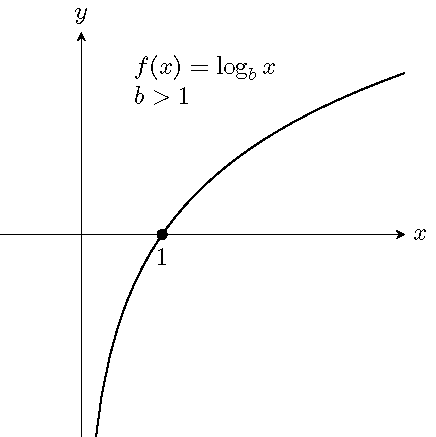
\includegraphics[scale=0.8]{figs/tikz-example-log-function-graph-1.png}

\columnbreak

  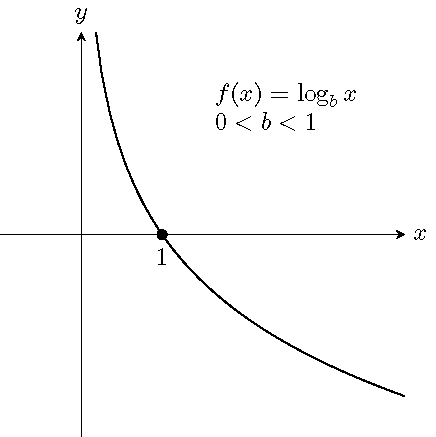
\includegraphics[scale=0.8]{figs/tikz-example-log-function-graph-2.png}
\end{multicols*}


\subsection{Commonand Natural
Logarithms}

A logarithmic function \(f(x)\) with base 10 is called the common
logarithmic function and denoted by \(f(x)=\log x\).

A logarithmic function \(f(x)\) with base the natural number \(e\) is
called the natural logarithmic function and denoted by \(f(x)=\ln x\).

\hypertarget{basic-properties-of-logarithms}{%
\subsection{Basic Properties of
Logarithms}\label{basic-properties-of-logarithms}}

When \(b>0\) and \(b\neq 1\), and \(x>0\), we have

\begin{enumerate}[sepno]
\item
  \(b^{\log_bx}=x\).
\item
  \(\log_b(b^x)=x\).
\item
  \(\log_bb=1\) and \(\log_b1=0\).
\end{enumerate}

\begin{example}

Convert between exponential and logarithmic forms.

\begin{enumerate}
\item
  \(\log x=\frac{1}{2}\)
\item
  \(3^{2x-1}=5\)
\end{enumerate}

\end{example}

\begin{example}

Evaluate the logarithms.

\begin{enumerate}
\item
  \(\log_42\)
\item
  \(10^{\log(\frac{1}{2})}\)
\item
  \(\log_5(e^0)\)
\end{enumerate}

\end{example}

\begin{example}

Find the domain of the function \(f(x)=\ln(2-3x)\).

\end{example}
\vspace*{6\baselineskip}

\hypertarget{properties-of-logarithms}{%
\subsection{Properties of Logarithms}\label{properties-of-logarithms}}

For \(M>0\), \(N>0\), \(b>0\) and \(b\neq 1\), we have

\begin{enumerate}[sepno]
\item
  (The product rule) \(\log_b(MN)=\log_bM+\log_bN\)
\item
  (The quotient rule) \(\log_b(\frac MN)=\log_bM-\log_bN\).
\item
  (The power rule) \(\log_b(M^p)=p\log_bM\), where \(p\) is any real
  number.
\item
  (The change-of-base property) \(\log_bM=\dfrac{\log_aM}{\log_ab}\),
  where \(a>0\) and \(a\neq 1\). In particular, \[
   \log_bM=\dfrac{\log M}{\log b} \quad\text{and}\quad \log_bM=\dfrac{\ln M}{\ln b}.
   \]
\end{enumerate}

\begin{example}

Expand and simplify the logarithm
\(\log_2\left(\frac{8\sqrt{y}}{x^3}\right)\).

\end{example}
\vspace*{6\baselineskip}

\begin{example}

Write the expression \(2\ln(x-1)-\ln(x^2+1)\) as a single logarithm.

\end{example}
\vspace*{6\baselineskip}

\begin{example}

Evaluate the logarithm \(\log_34\) and round it to the nearest tenth.

\end{example}
\vspace*{6\baselineskip}

\begin{example}

Simplify the logarithmic expression \[
\log_2(x^{\log 3})\log_32.
\]

\end{example}
\vspace*{6\baselineskip}

\subsection{Practice}

\begin{exercise}

Write each equation into equivalent exponential form.

\begin{enumerate}
\item
  \(\log_37=y\)
\item
  \(3=\log_b64\)
\item
  \(\log x=y\)
\item
  \(\ln(x-1)=c\)
\end{enumerate}

\end{exercise}

\begin{exercise}

Write each equation into equivalent logarithmic form.

\begin{enumerate}
\item
  \(7^x=10\)
\item
  \(b^5=2\)
\item
  \(e^{2y-1}=x\)
\item
  \(10^x=c^2+1\)
\end{enumerate}

\end{exercise}

\begin{exercise}

Evaluate.

\begin{enumerate}
\item
  \(\log_216\)
\item
  \(\log_93\)
\item
  \(\log 10\)
\item
  \(\ln 1\)
\end{enumerate}

\end{exercise}

\begin{exercise}

Evaluate.

\begin{enumerate}
\item
  \(e^{\ln 2}\)
\item
  \(\log 10^{\frac13}\)
\item
  \(\ln(\sqrt{e})\)
\item
  \(\log_2(\frac12)\)
\end{enumerate}

\end{exercise}

\begin{exercise}

Find the domain of the function \(f(x)=\log(x-5)\). Write in interval
notation.

\end{exercise}
\vspace*{6\baselineskip}

\begin{exercise}

Sketch the graph of each function and find its range.

\begin{enumerate}
\item
  \(f(x)=\log_2x\)
\item
  \(f(x)=\log_{\frac12} x\)
\end{enumerate}

\end{exercise}

\begin{exercise}

Expand the logarithm and simplify.

\begin{enumerate}
\item
  \(\log(100x)\)
\item
  \(\ln\left(\frac{10}{e^2}\right)\)
\item
  \(\log_b(\sqrt[3]{x})\)
\item
  \(\log_7(\frac{x^2\sqrt{y}}{z})\)
\end{enumerate}

\end{exercise}

\begin{exercise}

Expand the logarithm and simplify.

\begin{enumerate}
\item
  \(\log_b\sqrt{\frac{x^2y}{5}}\)
\item
  \(\ln(\sqrt[3]{(x^2+1)y^{-2}})\)
\item
  \(\log(x\sqrt{10x}-\sqrt{10x})\)
\end{enumerate}

\end{exercise}

\begin{exercise}

Write as a single logarithm.

\begin{enumerate}
\item
  \(\frac13\log x +\log y\)
\item
  \(\frac12\ln(x^2+1)-2\ln x\)
\item
  \(\frac13\log_2 x - 3\log_2(x+1)+1\)
\end{enumerate}

\end{exercise}

\begin{exercise}

Write as a single logarithm.

\begin{enumerate}
\item
  \(2\log(2x+1)-\frac12\log x\)
\item
  \(3\ln x - 5\ln y + \frac{1}{2}\ln z\)
\item
  \(3\log_3 x-2\log_3(1-x)+\frac13\log_3 (x^2+1)\).
\end{enumerate}

\end{exercise}

\begin{exercise}

Evaluate the logarithm and round it to the nearest hundredth.

\begin{enumerate}
\item
  \(\log_2 10\)
\item
  \(\log_3 5\)
\item
  \(\dfrac{1}{\log_52}\)
\item
  \(\log_45-\log_29\)
\end{enumerate}

\end{exercise}

\begin{exercise}

Simplify the logarithmic expression \[
\frac{\log_3(x^2)\log_y\sqrt{3}}{\log x}.
\]

\end{exercise}
